% Progress report — Machine Learning project, Bachelor in Applied Mathematics, IE University.
% Two pages of text excluding references. Compile: tectonic main.tex
\documentclass[9pt,twocolumn]{extarticle}
\usepackage[margin=0.75in,columnsep=0.25in]{geometry}
\usepackage[T1]{fontenc}
\usepackage[utf8]{inputenc}
\usepackage{lmodern}
\usepackage{microtype}
\usepackage{graphicx}
\usepackage{booktabs}
\usepackage{amsmath,amssymb}
\usepackage[numbers,sort&compress]{natbib}
\usepackage{titlesec}
\usepackage{enumitem}\setlist[itemize]{topsep=2pt,leftmargin=1.2em}
\usepackage[hidelinks]{hyperref}
\usepackage{xcolor}
\setcitestyle{sep={,}}
\setlength{\bibsep}{2pt}
\titlespacing*{\section}{0pt}{6pt plus 2pt minus 1pt}{3pt plus 1pt}
\titlespacing*{\subsection}{0pt}{5pt plus 2pt minus 1pt}{2pt plus 1pt}

\title{\vspace{-1.4em}\textbf{Learning the Country, Not the Camera:\\ Measuring and Explaining Contributor Shortcuts\\ in CNN-Based Country Recognition}\vspace{-0.6em}}
\author{Guillermo Gonz\'alez, Kwanhyung Kim\\[-2pt]
\small Bachelor in Applied Mathematics, IE University\\[-2pt]
\small Machine Learning \& Communication Skills --- Progress Report, Fall 2026}
\date{}

\begin{document}
\twocolumn[{\maketitle}]

\section*{Research question and design}
Can a convolutional network classify the country of a street-level photo from geographic
cues, or does it instead recognise the \emph{photographer}? Mapillary imagery in
OpenStreetView-5M (OSV-5M) \citep{astruc2024osv5m} is heavily contributed: most photos of a
country come from few recurring contributors whose cameras, mounts and colour profiles are
persistent identifiers \citep{lukas2006camera}, a textbook shortcut \citep{geirhos2020shortcut,
torralba2011unbiased, zech2018pneumonia}. Our question is quantitative: \emph{how much of the
accuracy of a country classifier is contributor identity, and where in the pipeline does it
enter?} We study it with ResNet-18 \citep{he2016resnet} on 32 countries (those with
$\geq$200 contributors), using a contributor-disjoint protocol: contributors are split
70/10/20 into train/val/test (stratified by main country), budgets per country are filled by
water-filling with a per-contributor cap, and two additional evaluation sets hold out entire
trips (linked by sequence or a $\sim$11\,km cell) of \emph{training} contributors. This yields
\emph{test} (12{,}800 images, 3{,}043 unseen contributors) and \emph{test$_{shared}$}
(12{,}559 images, 3{,}037 seen contributors; $\leq$400 images per country each), over a
training pool of 101{,}578 images from 11{,}132 contributors \citep{roberts2017crossvalidation,
kaufman2012leakage}. Images are centre-cropped to 4:3 (removing the 16:9/4:3 camera cue) and
stored at $128\times170$. We report balanced accuracy
$\mathrm{BA}=\tfrac1K\sum_k R_k$ (mean per-class recall; chance $1/K=3.1\%$) with 95\% CIs
from a bootstrap that resamples \emph{contributors}, not images \citep{field2007bootstrap};
the statistic of interest is the contributor gap
$\Delta=\mathrm{BA}(\text{test}_{shared})-\mathrm{BA}(\text{test})$, computed on paired
bootstrap draws so its interval is for the difference itself.

\section*{Models compared}
All models share the same data, splits and input resolution, forming an ablation ladder over
\emph{how much of the network is fitted to the contributors}:
\textbf{(i)~Linear probe.} Frozen ImageNet \citep{deng2009imagenet,kornblith2019transfer}
ResNet-18 features (512-d global average pool) with $L_2$-penalised softmax regression,
$\min_{W,b}\tfrac1n\sum_i \mathrm{CE}(W^\top f_i+b,y_i)+\lambda\lVert W\rVert_F^2$, fitted by
L-BFGS on 9{,}600 images (300 per country); $\lambda$ chosen on \emph{val} (unseen
contributors). \textbf{(ii)~Partial fine-tune} (CPU interim, no GPU access so far): the stem
and residual stages 1--2 stay frozen at ImageNet weights; stages 3--4 and the head train for
24 epochs of 20{,}480 images ($\approx$4.7 passes) with SGD (Nesterov, lr $0.02$ per 256
images scaled by batch, cosine decay after 0.5-epoch warm-up, weight decay $10^{-4}$ off
BatchNorm/bias), dropout 0.2, label-smoothed cross-entropy
($\varepsilon=0.1$: $q_y=1-\varepsilon+\varepsilon/K$, $q_{k\neq y}=\varepsilon/K$), random
resized crops (scale 0.6--1), and \emph{no} horizontal flip (mirroring swaps the driving
side). \textbf{(iii)~Staged data extension}: 261{,}572 additional images exist for our
countries under a 100-image-per-contributor cap (contributor concentration again), dealt into
three $\sim$87k chunks; each chunk is trained for five coverage epochs (every image exactly
once) from the previous best checkpoint, with inverse-frequency class weights and a 1{,}600
replay floor per country, giving cumulative distinct-image counts of
$189\mathrm{k}/276\mathrm{k}/363\mathrm{k}$.
\textbf{(iv)~$k$-nearest neighbours} on the same pooled features (z-scored on the gallery,
cosine, $k\in\{1,15\}$): a non-parametric alternative that also makes the shortcut directly
observable in retrieval.

\begin{table}[t]
\centering\scriptsize
\caption{Balanced accuracy (\%) on the two test protocols with 95\% contributor-clustered
CIs (test$_{shared}$ point estimates; CIs omitted for width) and the median great-circle
distance of \emph{errors} to the predicted country's centroid. Paired bootstrap vs.\ the
fine-tune: stage 3 test $+2.0$ $[1.4,2.5]$, gap $+1.6$ $[0.6,2.5]$.}
\label{tab:main}
\setlength{\tabcolsep}{3pt}
\begin{tabular}{lcccc}
\toprule
model & test & test$_{sh.}$ & $\Delta$ & err.\,km \\
\midrule
probe (frozen)  & 13.5 [12.8,14.3] & 13.7 & $+0.2$ [$-1.1,1.4$] & 5543 \\
fine-tune       & 28.7 [27.5,29.8] & 34.5 & $+5.8$ [$4.1,7.5$]   & 2439 \\
\;+ chunk 1     & 29.8 [28.6,31.0] & 36.8 & $+7.0$ [$5.2,8.8$]   & 2679 \\
\;+ chunk 2     & 30.1 [28.9,31.3] & 37.7 & $+7.6$ [$5.8,9.4$]   & 2852 \\
\;+ chunk 3     & \textbf{30.7} [29.4,31.9] & \textbf{38.0} & $+7.4$ [$5.6,9.2$] & 2865 \\
\midrule
15-NN (frozen)  & 9.7$^{\dagger}$  & 11.5$^{\dagger}$ & --- & --- \\
15-NN (stage 3) & 25.3$^{\dagger}$ & 32.8$^{\dagger}$ & --- & --- \\
\bottomrule
\end{tabular}
\\[2pt]{\footnotesize $^{\dagger}$top-1; gallery val $\to$ test, val$_{shared}\to$test$_{shared}$.}
\end{table}

\section*{Results: scaling buys little and widens the gap}
Table~\ref{tab:main} and Fig.~\ref{fig:main}a give the headline. Fitting the upper network
\emph{doubles} accuracy over frozen features (13.5$\to$28.7\% BA). Tripling the data again
adds only $+2.0$\,pp on unseen contributors while contributors already seen gain $+3.5$\,pp:
$\Delta$ widens from $+5.8$ to $+7.4$\,pp. Because new images are mostly \emph{more trips of
the same contributors}, scale adds contributor identity faster than geographic knowledge ---
consistent with the per-epoch curve, where the val gap
$\mathrm{BA}(\mathrm{val}_{shared})-\mathrm{BA}(\mathrm{val})$ stays near zero below
$\sim$37\% training accuracy (epochs 0--7) and grows to $+3$--$4$\,pp once the network fits
the training set ($>50\%$). Errors are not random either: confusions stay local
(Spain$\to$Italy, Czechia$\to$Poland), the worst classes are western-European (France 5\%),
and the median misclassification lands 5{,}543\,km from the truth for the probe but
2{,}439\,km after fine-tuning (correct answers sit $\sim$220\,km from their centroid):
fine-tuning mostly removes continent-level mistakes, and lifts top-3 test accuracy from 29.4
to 52.4\%. On frozen features a 15-NN reaches only 9.7\% top-1 (its trained head: 13.5\%);
after fine-tuning the gap narrows to 25.3 vs 30.7\%, so fine-tuning chiefly makes the
features \emph{metrically} country-ordered.

\begin{figure}[t]
\centering
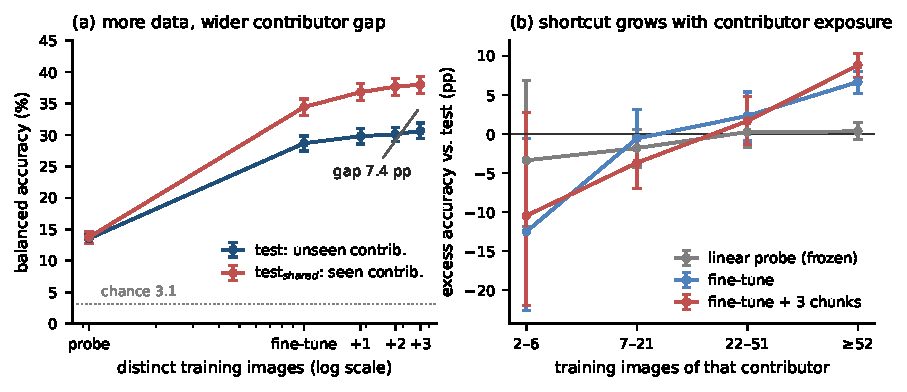
\includegraphics[width=\columnwidth]{figures/scaling_decomposition}
\caption{(a) Balanced accuracy versus distinct training images: the two protocols diverge as
data grows. (b) Country-adjusted excess accuracy on test$_{shared}$ (held-out trips of seen
contributors), binned by the contributor's number of training images, relative to the same
countries' accuracy on the disjoint test split; whiskers are 95\% contributor-bootstrap CIs.
Frozen features show no trend; fine-tuned models gain up to $+8.8$\,pp for the most-exposed
contributors.}
\label{fig:main}
\end{figure}

\section*{Anatomy of the shortcut: three convergent analyses}
\textbf{(1) Exposure dose--response.} If $\Delta$ were geography (seen contributors
photographing typical places), accuracy on their held-out trips would be flat in their
training exposure. Instead, we bin each test$_{shared}$ contributor by training images and
compute the country-adjusted excess
$E_B=\tfrac1{|B|}\sum_{i\in B}\big(\mathbf{1}[\hat y_i=y_i]-a_{c(i)}\big)$, where $a_c$ is the
same model's accuracy on country $c$ in the disjoint test split. The probe is flat
($+0.3$\,pp, CI $[-0.7,+1.4]$, for contributors with $\geq$52 images), whereas stage~3 gives
$+1.7$ $[-1.3,+4.8]$ at 22--51 images and $+8.8$\,pp $[+7.3,+10.3]$ at $\geq$52 images (median
exposure 99; 84\% of images; Fig.~\ref{fig:main}b). The advantage
is a \emph{memorisation dose--response}, not a sampling artefact.
\textbf{(2) Retrieval view.} In the 1-NN classifier (val$_{shared}$ gallery), 6.9\% of
test$_{shared}$ queries retrieve a photo by the \emph{same contributor} as nearest neighbour;
those queries are 90.6\% correct, the others 22.0\%. This single mechanism contributes
$0.069\times(0.906-0.220)\approx+4.7$\,pp of top-1 --- most of the +7.0\,pp top-1 gap
(37.6\% vs 30.7\%) --- and the comparison is within the same query set, so it is paired.
The same holds on frozen features (5.0\% of queries, then 89.6\% vs 7.0\% correct): the
retrieval cue is available to any photographer-clustered representation; only the
\emph{fitted classifier} turns it into an accuracy gap.
\textbf{(3) Feature-space verification.} We score pairs of \emph{test} images (contributors
never seen in training) by cosine similarity: same-photographer pairs from different
sequences versus different-photographer pairs from the same country, so country information
cannot help; AUC is 0.5 at chance. Frozen ImageNet features already separate photographers
(AUC $0.59$); fine-tuned features score $0.57$, with a 14\% nearest-neighbour
same-contributor rate against a 0.1\% random-pair chance. Photographer style is thus present
in the representation regardless of training --- yet the probe, built on the
\emph{more} photographer-decodable features, shows no gap and no exposure trend
(Fig.~\ref{fig:main}b). Decodable style alone does not create the shortcut; it appears only
when the classifier is fitted to specific contributors (analyses 1--2).

\section*{Problems encountered and decisions}
\begin{itemize}\itemsep1pt\parskip0pt
\item \emph{No GPU access yet.} Kaggle GPU quotas remain unconfigured, so we redesigned the
plan rather than the question: freeze stem and stages 1--2 (17 vs 10\,img/s), subsample
epochs to 20{,}480 images, make training resumable (checkpointed RNG and data order), and
train the data extension chunk-by-chunk. The GPU protocol (below) is unchanged and ready.
\item \emph{Static-pixel camera masks failed.} Temporally-static pixels should mark bonnets
and dashboards, but no pixel had across-photo std $<15$ for the 60 largest contributors, and
the few stable regions were roads, snow and sky --- country cues whose shapes would
themselves be fingerprints. Masks stay opt-in and frame-capped; instead we blank the bottom
20\% of every image, re-encode JPEG (quality 30--95) and jitter white
balance/brightness/contrast/saturation. Hue is deliberately \emph{not} jittered
(road-marking colour is a country cue); blanking---not cropping---keeps geometry identical.
This pipeline is implemented but awaits the GPU runs.
\item \emph{Warm restarts.} Stage~1 restarted at lr 0.01 and lost 3\,pp of val BA before
recovering; stages 2--3 restart at 0.004 with no dip. Stage~1 also introduced
inverse-frequency class weights together with new data, so that step does not cleanly
separate data from objective; the within-stage trajectories and the exposure analysis
(which is unaffected) carry the interpretation.
\item \emph{Data engineering.} 139{,}696 single JPEGs read out of 98 remote OSV-5M zips by
HTTP range requests (42\,min) instead of a 245\,GB download.
\end{itemize}

\section*{Plan to completion}
On GPU (Kaggle T4): the $2\times2$ design --- \{ImageNet, from-scratch\} $\times$
\{standard, fingerprint-removal\} --- testing whether bottom-band blanking and photometric
jitter close $\Delta$ and at what cost in disjoint-test accuracy; end-to-end fine-tuning; a
wider $\lambda$ grid for the probe (its optimum sits at the grid edge); Grad-CAM
qualitative analysis; and possibly a domain-adversarial contributor penalty
\citep{ganin2016dann}. The final report adds per-class and confusion analysis and the
interactive ``Dashcam Duel'' demonstration.

\footnotesize\textit{Data: OSV-5M, CC-BY-SA-4.0 \citep{astruc2024osv5m}; code, scripts and run artifacts:
\url{https://github.com/LaGuadana/country-not-camera}. AI use: ZCode (GLM) assisted with pipeline/analysis code and
produced a first draft of this text, which the authors revised, verified claim by claim
against the run artifacts, and take full responsibility for.}

\bibliographystyle{plainnat}
\bibliography{references}
\end{document}
